\documentclass[10pt]{beamer}
\usetheme{Warsaw}
\usepackage[T1]{fontenc}
\usepackage[utf8]{inputenc}
\usepackage{chronosys}
\usepackage{graphicx}
\usepackage{multicol} % Pour les colonnes multiples

\begin{document}

% Page de titre avec les logos
\begin{frame}
\frametitle{KINETIC AND BUILDING LOD2}
\begin{figure}
    % Première ligne de logos
    \begin{minipage}{0.33\textwidth}
        \centering
        
\includegraphics[width=0.6\textwidth]{../image/logo_irma.png}
    \end{minipage}%
    \begin{minipage}{0.33\textwidth}
        \centering
        
\includegraphics[width=0.6\textwidth]{../image/logo-numpex-web-2.png}
    \end{minipage}%
    \begin{minipage}{0.33\textwidth}
        \centering
        
\includegraphics[width=0.6\textwidth]{../image/logo-ufr-mathinfo-unistra-1.jpg}
    \end{minipage}
    
    \vspace{0.5cm} % Espacement entre les deux lignes
    
    % Deuxième ligne de logos
    \begin{minipage}{0.33\textwidth}
        \centering
        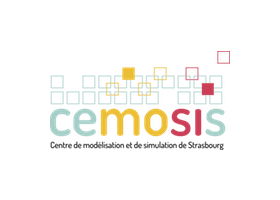
\includegraphics[width=0.6\textwidth]{../image/logoCemosis-square-e1469167314407.png}
    \end{minipage}%
    \begin{minipage}{0.33\textwidth}
        \centering
        
\includegraphics[width=0.6\textwidth]{../image/HiDALGO2 - logo - color - RGB.jpg}
    \end{minipage}%
    \begin{minipage}{0.33\textwidth}
        \centering
        
\includegraphics[width=0.6\textwidth]{../image/G_logo-inria-rouge-reduce_inr_logo_rouge_1080x608.jpg}
    \end{minipage}
    
\end{figure}

\vspace{0.5cm} 

Intern: Demuth Axel \\
Supervisor: Vincent Chabannes, Pierre Alliez, Florent Lafarge

\end{frame}

\begin{frame}
    \frametitle{Table of Contents}
    \begin{multicols}{2} % Diviser la page en deux colonnes
        \tableofcontents
    \end{multicols}
    \end{frame}


\section{Introduction}
\begin{frame}{Introduction}
    \subsection{Context}
\end{frame}

\begin{frame}{Issue with Kinetic Algorithm}
    \subsection{Issue with Kinetic Algorithm}
\end{frame}

% Objectives
\begin{frame}{Objectives}
    \subsection{Objectives}
    \begin{itemize}
        \item Check the validity of the Mesh
        \item Create a workflow for automatic generation using KSR Algorithm
        \item Keep the correspondence of surfaces between both meshes
        \item Run some simulations using the Feel++ library
    \end{itemize}
\end{frame}

% CGAL
\begin{frame}{CGAL}
    \subsection{CGAL}
    \begin{itemize}
        \item C++ library for geometric calculations, providing data structures for mesh generation and manipulation.
    \end{itemize}
    \vspace{0.5cm}
    The main packages utilized are:
    \begin{itemize}
        \item \texttt{CGAL::Polygon\_mesh\_processing}
        \item \texttt{CGAL::Surface\_mesh}
        \item \texttt{CGAL::Point\_set\_processing}
        \item \texttt{CGAL::IO\_streams}
        \item \texttt{CGAL::AABB\_tree}
    \end{itemize}
    
\end{frame}


\section{Data}
\subsection{Files Format}
\begin{frame}{File Format}
\begin{itemize}
    \item IFC 
    \item CityGML
    \item STL 
    \item OBJ
    \item OFF
    \item Ply
    \item Msh
\end{itemize}
\end{frame}

\subsection{Software and Data}
\begin{frame}{Software}
    \begin{itemize}
        \item Github : Platforme for collaborating work on a project
        \item Visual Studio Code : Versatil tools for coding with various extensions
        \item Paraview : Open-source data analysis and visualisation
        \item Meshlab : A tool for processing,editing,visualisation of 3D mesh
        \item GMSH : a 3D finite element mesh generator
    \end{itemize}

\end{frame}

\begin{frame}{Data}
    
\end{frame}


\section{Methodology}
\subsection{Kinetic}
\begin{frame}{Kinetic}
    
\end{frame}

\subsection{preprocessing}
\begin{frame}{preprocessing}  
\end{frame}

\subsection{labelling}
\begin{frame}{Labelling}
\end{frame}

\subsection*{Metric}
\begin{frame}{Metric}
    
\end{frame}

\section{Implementation}
\subsection{Contribution to Ktirio library}
\begin{frame}
    
\end{frame}

\subsection{test}
\begin{frame}{test}
\end{frame}

\section{Result}
\subsection{Point cloud generation Result}
\begin{frame}{Point cloud}
    
\end{frame}

\subsection{Self Intersection Result}
\begin{frame}{Self Intersection fixing}
    
\end{frame}

\subsection{Performance}
\begin{frame}{Performance}
    
\end{frame}

\section{Conclusion}
\begin{frame}{Conclusion}
    
\end{frame}

\section{Refereces}
\begin{frame}{bib}
    
\end{frame}

\end{document}
